\documentclass{article}
\pagestyle{empty}
\usepackage[margin=5mm]{geometry}

%\usepackage{mathptmx}
%\usepackage{fontspec}
%\usepackage{mathspec}
%\setmathsfont(Digits,Latin,Greek){TeX Gyre Pagella}
\usepackage{unicode-math} % https://tex.stackexchange.com/questions/96024/how-to-use-system-font-for-equation-in-xelatex
\setmainfont[AutoFakeSlant,AutoFakeBold]{TeX Gyre Pagella}
\setmathfont{Asana Math}

\usepackage{pgfplots}
\pgfplotsset{
    compat=1.14,
    axis lines=center,
    scale only axis=true,
    every axis y label/.style={
        at={(ticklabel* cs:1)}, anchor=south, font=\tiny
    },
    every axis x label/.style={
        at={(ticklabel* cs:1)}, anchor=west, font=\tiny
    },
    every axis title/.append style={
        at={(0,1)},
        anchor=north west,
        font=\footnotesize,
        xshift=3pt, yshift=0pt
    },
    every tick label/.append style={
        font=\tiny
    },
    every axis legend/.append style={
        font=\tiny,
        fill=none,
        draw=none
    },
    xtick distance=1,
    restrict y to domain=-100:100,
    unbounded coords=jump,
}
\tikzset{>=latex}

\begin{document}
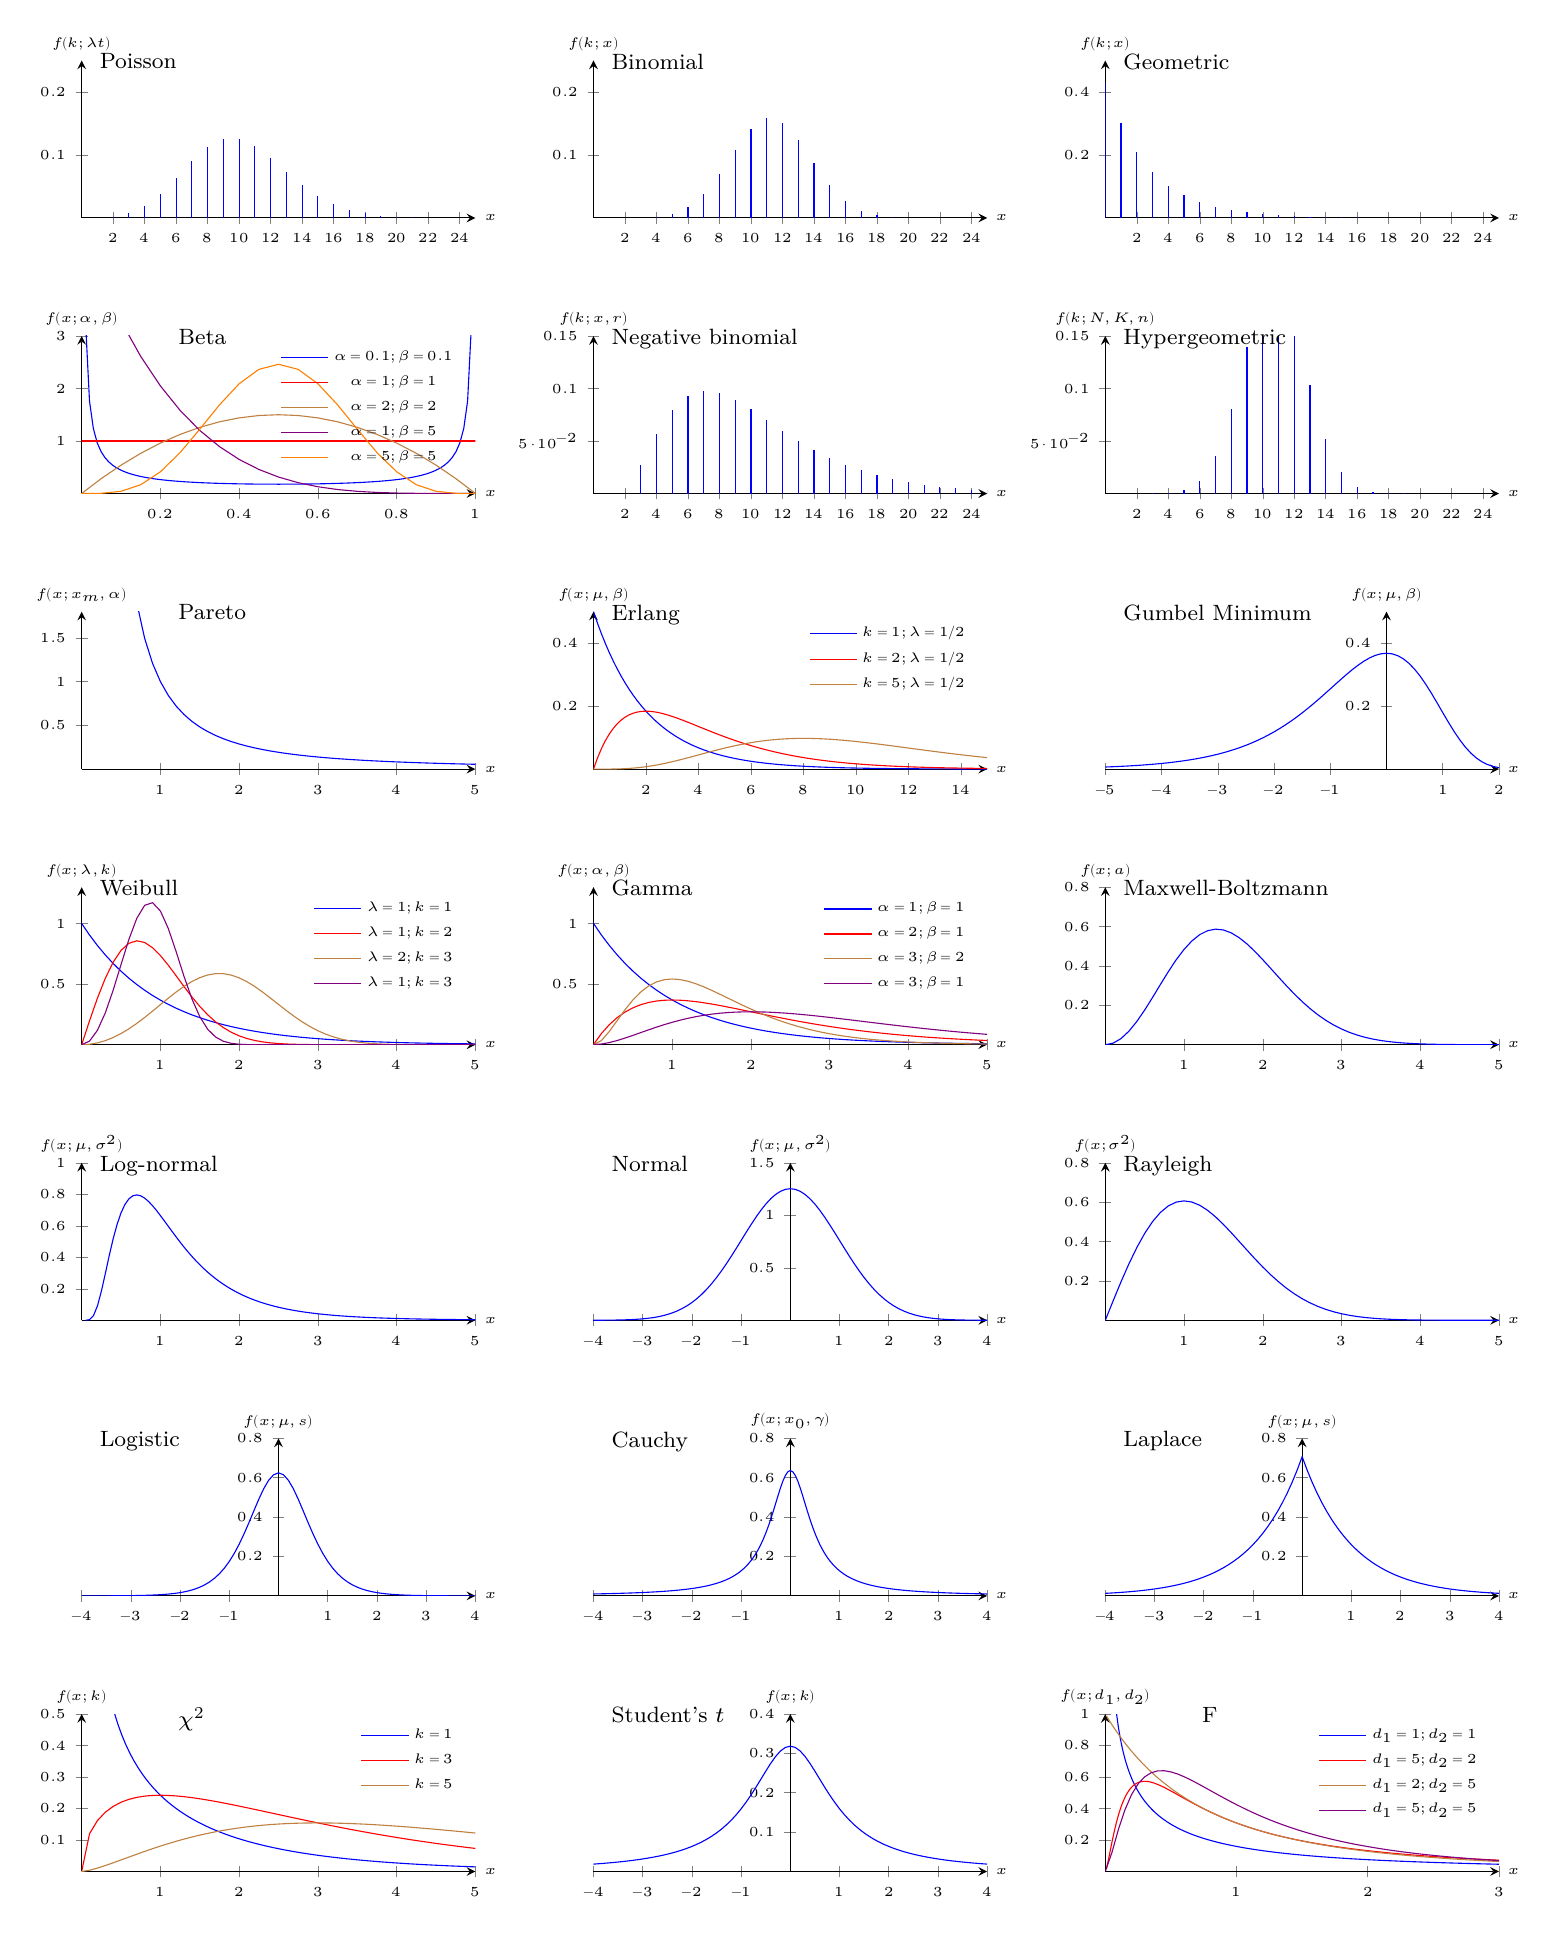
\begin{tikzpicture}

% Chi-squared
\begin{axis}[
    name=plotChiSquared,
    height=2cm, width=5cm,
    %axis equal=true,
    title=$\chi^2$,
    title style={at={(0.2,1)}},
    xlabel={$x$}, ylabel={$f(x;k)$},
    legend entries={$k=1$, $k=3$, $k=5$},
    ymin=0, ymax=0.5, xmin=0, xmax=5,
    xtick distance=1,
    ytick distance=0.1,
    at={(0cm, 0cm)}, anchor=south
]
  \addplot[blue, samples=101, domain=0.01:5] {x^(-0.5) * exp(-x/2) / (2^(0.5) * 1.772454)};
  \addplot[red, samples=101] {x^(0.5) * exp(-x/2) / (2^(1.5) * 0.886227)};
  \addplot[brown, samples=101] {x^(1.5) * exp(-x/2) / (2^(2.5) * 1.32934)};
\end{axis};

% Student's t
\begin{axis}[
    name=plotStudentT,
    height=2cm, width=5cm,
    %axis equal=true,
    title=Student's $t$,
    xlabel={$x$}, ylabel={$f(x;k)$},
    ymin=0, ymax=0.4, xmin=-4, xmax=4,
    xtick distance=1,
    ytick distance=0.1,
    at={(65mm, 0cm)}, anchor=south
]
    \addplot[blue, samples=101] {1/sqrt(pi)/1.772454 * (1+x^2)^(-1)};
\end{axis};

% F
\begin{axis}[
    name=plotF,
    height=2cm, width=5cm,
    %axis equal=true,
    title=F,
    title style={at={(0.2,1)}},
    xlabel={$x$}, ylabel={$f(x;d_1,d_2)$},
    legend entries={$d_1=1;d_2=1$, $d_1=5;d_2=2$, $d_1=2;d_2=5$, $d_1=5;d_2=5$},
    ymin=0, ymax=1, xmin=0, xmax=3,
    xtick distance=1,
    at={(13cm, 0cm)}, anchor=south
] % d1,d2 = 1,1 ; 3,1 ; 1,3 ; 5,2 ; 2,5 ; 5,5
  \addplot[blue, samples=201, domain=0.01:3] {sqrt(x/(x+1)^2)/(x*pi)};
  \addplot[red, samples=201, domain=0.01:3] {sqrt(4*((5*x)^5)/(5*x+2)^7)/(x*0.4)};
  \addplot[brown, samples=201, domain=0.01:3] {sqrt(3125*((2*x)^2)/(2*x+5)^7)/(x*0.4)};
  \addplot[violet, samples=201] {sqrt(3125*((5*x)^5)/(5*x+5)^(10))/(x*0.073631)};
\end{axis};

% ---------------------------

% LOGISTIC
\begin{axis}[
    name=plotLogistic,
    height=2cm, width=5cm,
    %axis equal=true,
    title=Logistic,
    xlabel={$x$}, ylabel={$f(x;\mu, s)$},
    xmin=-4, xmax=4, ymin=0, ymax=0.8,
    at={(0cm, 35mm)}, anchor=south
]
  \addplot[blue, samples=101] {exp(-x/0.4)/(0.4*(1+exp(-x/0.4))^2)};
\end{axis};

% CAUCHY
\begin{axis}[
    name=plotCauchy,
    height=2cm, width=5cm,
    %axis equal=true,
    title=Cauchy,
    xlabel={$x$}, ylabel={$f(x;x_0, \gamma)$},
    xmin=-4, xmax=4, ymin=0, ymax=0.8,
    at={(65mm, 35mm)}, anchor=south
]
  \addplot[blue, samples=201] {1/(pi*0.5*(1+(x/0.5)^2))};
\end{axis};

% LAPLACE
\begin{axis}[
    name=plotLaplace,
    height=2cm, width=5cm,
    %axis equal=true,
    title=Laplace,
    xlabel={$x$}, ylabel={$f(x;\mu, s)$},
    xmin=-4, xmax=4, ymin=0, ymax=0.8,
    at={(13cm, 35mm)}, anchor=south
]
    \addplot[blue, samples=101] {sqrt(1/2) * exp(-abs(x))};
\end{axis};

% ---------------------------

% LOGNORMAL
\begin{axis}[
    name=plotLognormal,
    height=2cm, width=5cm,
    %axis equal=true,
    title=Log-normal,
    xlabel={$x$}, ylabel={$f(x;\mu, \sigma^2)$},
    xmin=0, ymin=0, ymax=1,
    at={(0cm, 7cm)}, anchor=south
]
  \addplot[blue, samples=201] {1/(sqrt(2*pi)*0.6*x) * exp(-ln(x)^2/(2*0.36))};
\end{axis};

% NORMAL
\begin{axis}[
    name=plotNormal,
    height=2cm, width=5cm,
    %axis equal=true,
    title=Normal,
    xlabel={$x$}, ylabel={$f(x;\mu,\sigma^2)$},
    ymin=0, ymax=1.5, xmin=-4, xmax=4,
    at={(65mm,7cm)}, anchor=south
]
  \addplot[blue, samples=101] {sqrt(1/2*pi) * exp(-x^2/2)};
\end{axis};

% RAYLEIGH
\begin{axis}[
    name=plotRayleigh,
    height=2cm, width=5cm,
    %axis equal=true,
    title=Rayleigh,
    xlabel={$x$}, ylabel={$f(x;\sigma^2)$},
    xmin=0, ymin=0, ymax=0.8,
    at={(13cm, 7cm)}, anchor=south
]
  \addplot[blue, samples=101] {x * exp(-x^2/2)};
\end{axis};

% ---------------------------

% WEIBULL
\begin{axis}[
    name=plotWeibull,
    height=2cm, width=5cm,
    %axis equal=true,
    title=Weibull,
    xlabel={$x$}, ylabel={$f(x;\lambda, k)$},
    legend entries={$\lambda=1;k=1$, $\lambda=1;k=2$, $\lambda=2;k=3$, $\lambda=1;k=3$},
    ymin=0, ymax=1.3, xmin=0, xmax=5,
    at={(0cm, 105mm)}, anchor=south
]
  \addplot[blue, samples=101] {exp(-x)};
  \addplot[red, samples=101] {2*x*exp(-x^2)};
  \addplot[brown, samples=101] {(3/2)*((x/2)^2)*exp(-(x/2)^3)};
  \addplot[violet, samples=101] {3*(x^2)*exp(-x^3)};
\end{axis};

% GAMMA
\begin{axis}[
    name=plotGamma,
    height=2cm, width=5cm,
    %axis equal=true,
    title=Gamma,
    xlabel={$x$}, ylabel={$f(x;\alpha,\beta)$},
    legend entries={$\alpha=1;\beta=1$, $\alpha=2;\beta=1$, $\alpha=3;\beta=2$, $\alpha=3;\beta=1$},
    ymin=0, ymax=1.3, xmin=0, xmax=5,
    at={(65mm, 105mm)}, anchor=south
]
  \addplot[blue, samples=101] {exp(-x)};
  \addplot[red, samples=101] {x*exp(-x)};
  \addplot[brown, samples=101] {(8/2)*(x^2)*exp(-2*x)};
  \addplot[violet, samples=101] {(1/2)*(x^2)*exp(-x)};
\end{axis};

% MAXWELL-BOLTZMANN
\begin{axis}[
    name=plotMaxwell,
    height=2cm, width=5cm,
    %axis equal=true,
    title=Maxwell-Boltzmann,
    xlabel={$x$}, ylabel={$f(x;a)$},
    xmin=0, ymin=0, ymax=0.8,
    at={(13cm, 105mm)}, anchor=south
]
  \addplot[blue, samples=101] {sqrt(2/pi) * x^2 * exp(-x^2/2)};
\end{axis};

% ---------------------------

% PARETO
\begin{axis}[
    name=plotPareto,
    height=2cm, width=5cm,
    %axis equal=true,
    title=Pareto,
    title style={at={(0.2,1)}},
    xlabel={$x$}, ylabel={$f(x;x_m, \alpha)$},
    xmin=0, ymin=0, ymax=1.8,
    at={(0cm, 14cm)}, anchor=south
]
  \addplot[blue, samples=101] {1/x^(1.8)};
\end{axis};

% ERLANG
\begin{axis}[
    name=plotErlang,
    height=2cm, width=5cm,
    %axis equal=true,
    title=Erlang,
    xlabel={$x$}, ylabel={$f(x;\mu,\beta)$},
    legend entries={$k=1;\lambda=1/2$, $k=2;\lambda=1/2$, $k=5;\lambda=1/2$},
    ymin=0, ymax=0.5, xmin=0, xmax=15,
    xtick distance=2,
    at={(65mm, 14cm)}, anchor=south
]
  \addplot[blue, samples=101, domain=0:15] {0.5*exp(-x/2)};
  \addplot[red, samples=101, domain=0:15] {(0.5)^2*x*exp(-x/2)};
  \addplot[brown, samples=101, domain=0:15] {(0.5)^5*x^4*exp(-x/2)/(4!)};
\end{axis};

% GUMBEL MINIMUM
\begin{axis}[
    name=plotGumbel,
    height=2cm, width=5cm,
    %axis equal=true,
    %title style={at={(1,1)}, anchor=north east, xshift=-5pt},
    title=Gumbel Minimum,
    xlabel={$x$}, ylabel={$f(x;\mu,\beta)$},
    ymin=0, ymax=0.5, xmin=-5, xmax=2,
    at={(13cm, 14cm)}, anchor=south
]
  \addplot[blue, samples=101] {exp(x-exp(x))};
\end{axis};

% ---------------------------

% BETA
\begin{axis}[
    name=plotBeta,
    height=2cm, width=5cm,
    %axis equal=true,
    title=Beta,
    title style={at={(0.2,1)}},
    xlabel={$x$}, ylabel={$f(x;\alpha,\beta)$},
    legend entries={$\alpha=0.1;\beta=0.1$, $\alpha=1;\beta=1$, $\alpha=2;\beta=2$, $\alpha=1;\beta=5$, $\alpha=5;\beta=5$},
    ymin=0, ymax=3, xmin=0, xmax=1,
    xtick distance=0.2,
    at={(0cm, 175mm)}, anchor=south
]
  \addplot[blue, samples=101, domain=0.01:0.99] {0.0507*x^(-0.9)*(1-x)^(-0.9)};
  \addplot[red, samples=101] {1.0};
  \addplot[brown, samples=201] {6*x*(1-x)};
  \addplot[violet, samples=201] {5*(1-x)^4};
  \addplot[orange, samples=201] {630*x^4*(1-x)^4};
\end{axis};

% NEGATIVE BINOMIAL 
\begin{axis}[
    name=plotNegBinom,
    height=2cm, width=5cm,
    %axis equal=true,
    title=Negative binomial,
    xlabel={$x$}, ylabel={$f(k;x,r)$},
    ymin=0, ymax=0.15, xmin=0, xmax=25,
    xtick distance=2,
    at={(65mm, 175mm)}, anchor=south
]
    \addplot[blue, ycomb] coordinates {
        (3,0.027000)
        (4,0.056700)
        (5,0.079380)
        (6,0.092610)
        (7,0.097240)
        (8,0.095296)
        (9,0.088943)
        (10,0.080048)
        (11,0.070042)
        (12,0.059925)
        (13,0.050337)
        (14,0.041643)
        (15,0.034008)
        (16,0.027468)
        (17,0.021974)
        (18,0.017433)
        (19,0.013729)
        (20,0.010741)
        (21,0.008354)
        (22,0.006463)
        (23,0.004977)
        (24,0.003815)
        (25,0.002914)
    };
\end{axis};

% HYPERGEOMETRIC
\begin{axis}[
    name=plotHypergeo,
    height=2cm, width=5cm,
    %axis equal=true,
    title=Hypergeometric,
    xlabel={$x$}, ylabel={$f(k;N,K,n)$},
    ymin=0, ymax=0.15, xmin=0, xmax=25,
    xtick distance=2,
    at={(13cm, 175mm)}, anchor=south
]
    \addplot[blue, ycomb] coordinates {
        (0,0.000000)
        (1,0.000000)
        (2,0.000006)
        (3,0.000071)
        (4,0.000557)
        (5,0.003043)
        (6,0.012075)
        (7,0.035754)
        (8,0.080447)
        (9,0.139292)
        (10,0.187208)
        (11,0.196372)
        (12,0.161219)
        (13,0.103641)
        (14,0.052076)
        (15,0.020367)
        (16,0.006159)
        (17,0.001427)
        (18,0.000250)
        (19,0.000032)
        (20,0.000003)
        (21,0.000000)
        (22,0.000000)
        (23,0.000000)
        (24,0.000000)
        (25,0.000000)
    };
\end{axis};

% ---------------------------

% POISSON
\begin{axis}[
    name=plotPoisson,
    height=2cm, width=5cm,
    %axis equal=true,
    title=Poisson,
    xlabel={$x$}, ylabel={$f(k;\lambda t)$},
    ymin=0, ymax=0.25, xmin=0, xmax=25,
    xtick distance=2,
    at={(0cm, 21cm)}, anchor=south
]
    \addplot[blue, ycomb] coordinates {
        (0,0.000045)
        (1,0.000454)
        (2,0.002270)
        (3,0.007567)
        (4,0.018917)
        (5,0.037833)
        (6,0.063055)
        (7,0.090079)
        (8,0.112599)
        (9,0.125110)
        (10,0.125110)
        (11,0.113736)
        (12,0.094780)
        (13,0.072908)
        (14,0.052077)
        (15,0.034718)
        (16,0.021699)
        (17,0.012764)
        (18,0.007091)
        (19,0.003732)
        (20,0.001866)
        (21,0.000889)
        (22,0.000404)
        (23,0.000176)
        (24,0.000073)
        (25,0.000029)
    };
\end{axis};

% BINOMIAL
\begin{axis}[
    name=plotBinomial,
    height=2cm, width=5cm,
    %axis equal=true,
    title=Binomial,
    xlabel={$x$}, ylabel={$f(k;x)$},
    ymin=0, ymax=0.25, xmin=0, xmax=25,
    xtick distance=2,
    at={(65mm, 21cm)}, anchor=south
]
    \addplot[blue, ycomb] coordinates {
        (0,0.0000)
        (1,0.0000)
        (2,0.0001)
        (3,0.0004)
        (4,0.0018)
        (5,0.0063)
        (6,0.0172)
        (7,0.0381)
        (8,0.0701)
        (9,0.1084)
        (10,0.1419)
        (11,0.1583)
        (12,0.1511)
        (13,0.1236)
        (14,0.0867)
        (15,0.0520)
        (16,0.0266)
        (17,0.0115)
        (18,0.0042)
        (19,0.0013)
        (20,0.0003)
        (21,0.0001)
        (22,0.0000)
        (23,0.0000)
        (24,0.0000)
        (25,0.0000)
    };
\end{axis};

% GEOMETRIC
\begin{axis}[
    name=plotGeometric,
    height=2cm, width=5cm,
    %axis equal=true,
    title=Geometric,
    xlabel={$x$}, ylabel={$f(k;x)$},
    ymin=0, ymax=0.5, xmin=0, xmax=25,
    xtick distance=2,
    at={(13cm, 21cm)}, anchor=south
]
    \addplot[blue, ycomb] coordinates {
        (0,0.428571)
        (1,0.300000)
        (2,0.210000)
        (3,0.147000)
        (4,0.102900)
        (5,0.072030)
        (6,0.050421)
        (7,0.035295)
        (8,0.024706)
        (9,0.017294)
        (10,0.012106)
        (11,0.008474)
        (12,0.005932)
        (13,0.004152)
        (14,0.002907)
        (15,0.002035)
        (16,0.001424)
        (17,0.000997)
        (18,0.000698)
        (19,0.000489)
        (20,0.000342)
        (21,0.000239)
        (22,0.000168)
        (23,0.000117)
        (24,0.000082)
        (25,0.000057)
    };
\end{axis};

% ---------------------------

%\draw[->] (plotNormal.east)--(plotRayleigh.outer west) node[draw=none,fill=none,midway,below] {$L^2$};
%\draw[->] (plotNormal.north east)--(plotMaxwell.south west) node[draw=none,fill=none,midway,below] {$L^2$};
%\draw[->] (plotNormal.west)--(plotLognormal.east) node[draw=none,fill=none,midway,below] {$\log(X)$};
%\draw[->] (plotNormal.outer south west)--(plotChiSquared.north east) node[draw=none,fill=none,near end,right] {$\sum z_i$};
%\draw[->] (plotNormal.outer south)--(plotCauchy.outer north) node[draw=none,fill=none,midway,right] {$X_1/X_2$};
%\draw[<->,dashed] (plotNormal.outer south east)--(plotLaplace.outer north west);
%\draw[<->,dashed] (plotErlang.outer south)--(plotGamma.outer.north);
%\draw[<->,dashed] (plotErlang.east)--(plotGumbel.west);

\end{tikzpicture}
\end{document}
